\section{Comparative Analysis of Strategies}
\label{sec:eval-comparative}

We compare four \textit{Invox} strategies—S1 (single-pass), S2 (iterative per-field), S3 (full-document consensus), and S4 (per-field consensus)—along \textbf{semantic accuracy} (R2), \textbf{latency} (R6), and \textbf{modularity} (R5). 
All numbers below use the few-shot, original MUC-4 setting for each strategy.

\subsection*{Quantitative Comparison}

% Add to your preamble:
% \usepackage{pgfplots}
% \pgfplotsset{compat=1.18}

\begin{figure}[h]
\centering
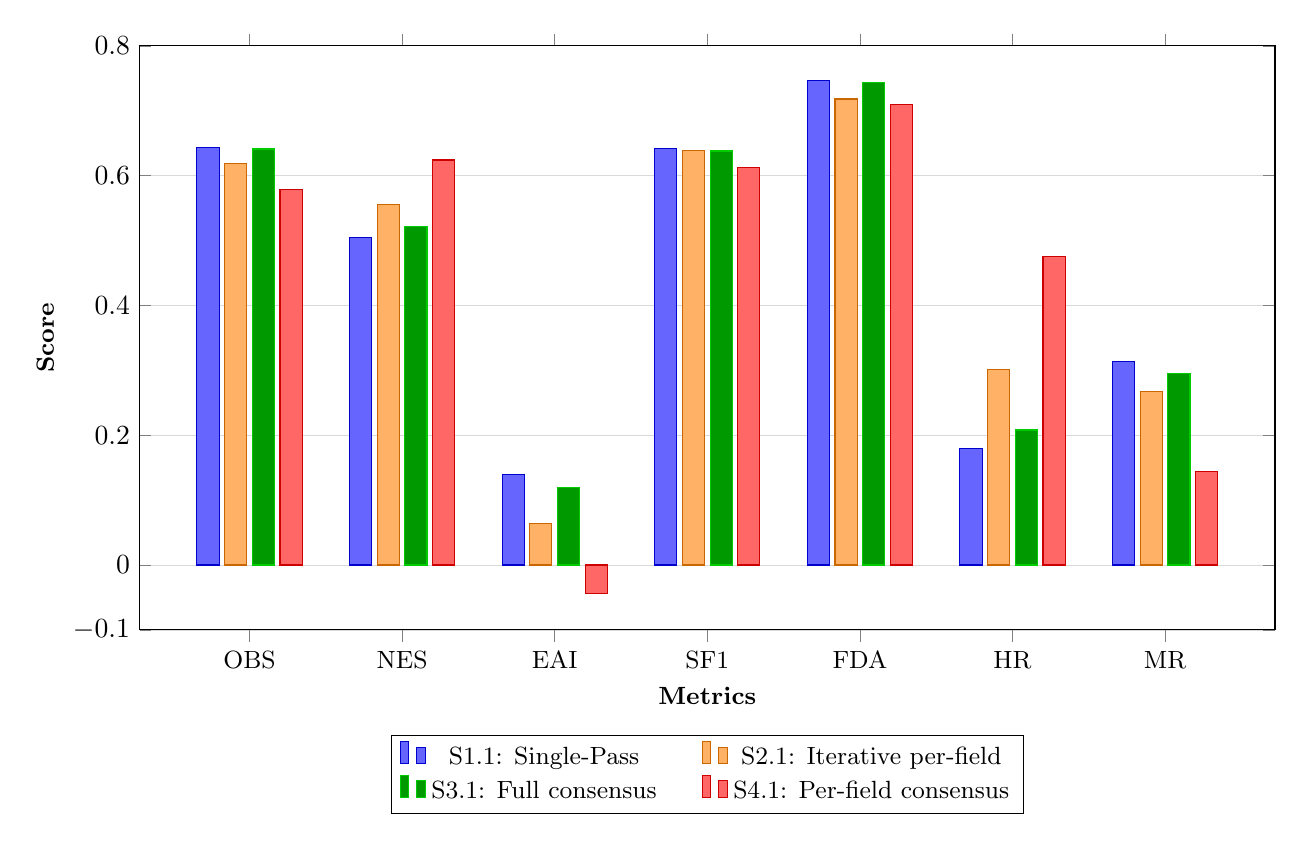
\begin{tikzpicture}
  \begin{axis}[
    width=16cm,
    height=9cm,
    ybar,
    bar width=8pt,
    ylabel={Score},
    ylabel style={font=\small\bfseries},
    xlabel={Metrics},
    xlabel style={font=\small\bfseries},
    symbolic x coords={OBS, NES, EAI, SF1, FDA, HR, MR},
    xtick=data,
    xticklabel style={font=\small},
    ymin=-0.1,
    ymax=0.8,
    ytick={-0.1, 0, 0.2, 0.4, 0.6, 0.8},
    ymajorgrids=true,
    grid style={line width=0.3pt, draw=gray!30},
    legend style={
      at={(0.5,-0.18)},
      anchor=north,
      legend columns=2,
      font=\small,
      /tikz/every even column/.append style={column sep=0.5cm}
    },
    enlarge x limits=0.12,
  ]
  
  % S1.1: Single-Pass - Blue
  \addplot[fill=blue!60, draw=blue!80!black] coordinates {
    (OBS, 0.644)
    (NES, 0.504)
    (EAI, 0.140)
    (SF1, 0.642)
    (FDA, 0.746)
    (HR, 0.180)
    (MR, 0.313)
  };
  \addlegendentry{S1.1: Single-Pass}
  
  % S2.1: Iterative per-field - Orange
  \addplot[fill=orange!60, draw=orange!80!black] coordinates {
    (OBS, 0.619)
    (NES, 0.555)
    (EAI, 0.064)
    (SF1, 0.639)
    (FDA, 0.718)
    (HR, 0.301)
    (MR, 0.267)
  };
  \addlegendentry{S2.1: Iterative per-field}
  
  % S3.1: Full consensus - Green
  \addplot[fill=green!60!black, draw=green!80!black] coordinates {
    (OBS, 0.641)
    (NES, 0.521)
    (EAI, 0.120)
    (SF1, 0.638)
    (FDA, 0.743)
    (HR, 0.208)
    (MR, 0.295)
  };
  \addlegendentry{S3.1: Full consensus}
  
  % S4.1: Per-field consensus - Red
  \addplot[fill=red!60, draw=red!80!black] coordinates {
    (OBS, 0.579)
    (NES, 0.624)
    (EAI, -0.044)
    (SF1, 0.613)
    (FDA, 0.709)
    (HR, 0.476)
    (MR, 0.144)
  };
  \addlegendentry{S4.1: Per-field consensus}
  
  \end{axis}
\end{tikzpicture}
\caption{Macro comparison (clean text; few-shot original).}
\label{fig:strategy-comparison-bar}
\end{figure}

\noindent\textit{Embedding alignment (baseline regime):} Chamfer (sym.) — S1.1: 0.642; S2.1: 0.639; S3.1: 0.638; S4.1: 0.613.

\subsection*{Latency Comparison (R6)}
\begin{figure}[h]
\centering
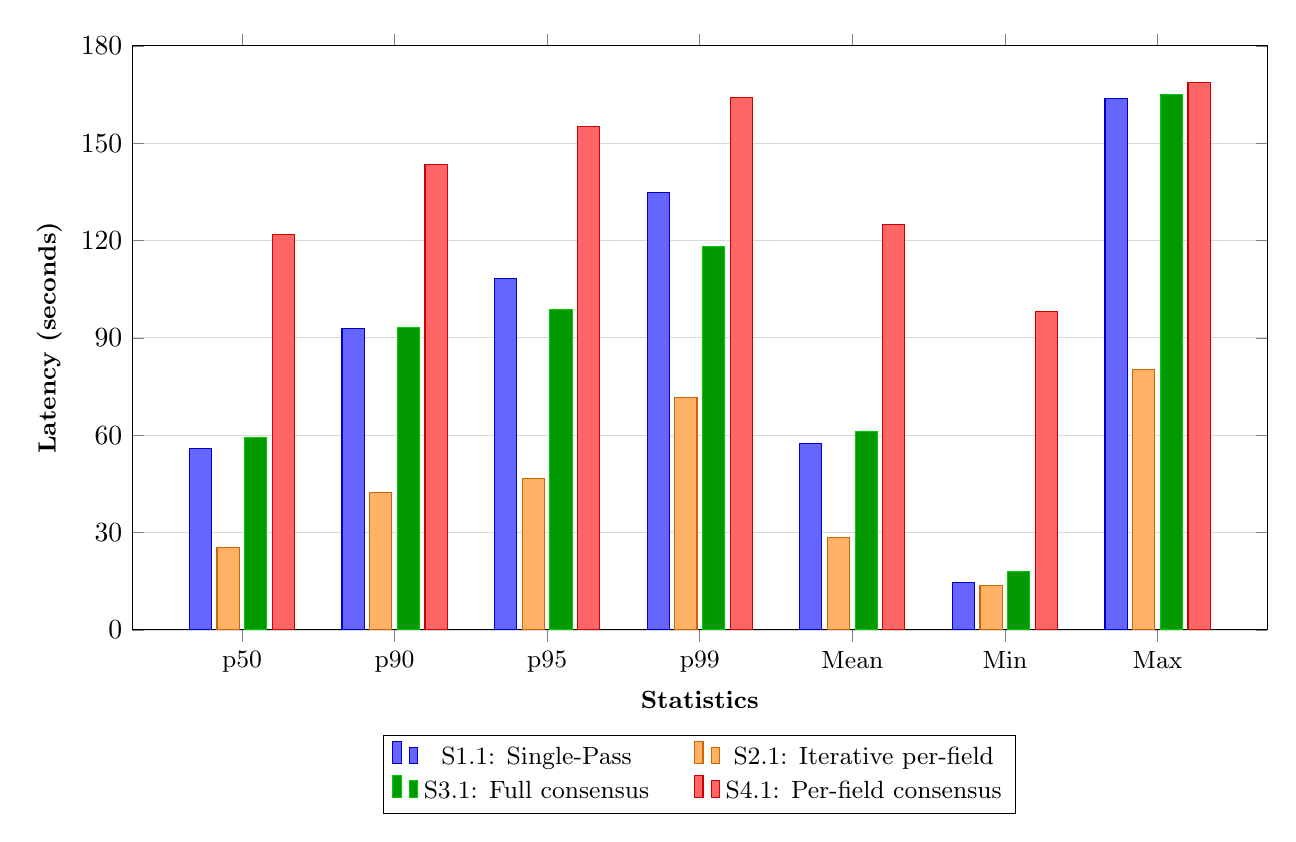
\begin{tikzpicture}
  \begin{axis}[
    width=16cm,
    height=9cm,
    ybar,
    bar width=8pt,
    ylabel={Latency (seconds)},
    ylabel style={font=\small\bfseries},
    xlabel={Statistics},
    xlabel style={font=\small\bfseries},
    symbolic x coords={p50, p90, p95, p99, Mean, Min, Max},
    xtick=data,
    xticklabel style={font=\small},
    ymin=0,
    ymax=180,
    ytick={0, 30, 60, 90, 120, 150, 180},
    ymajorgrids=true,
    grid style={line width=0.3pt, draw=gray!30},
    legend style={
      at={(0.5,-0.18)},
      anchor=north,
      legend columns=2,
      font=\small,
      /tikz/every even column/.append style={column sep=0.5cm}
    },
    enlarge x limits=0.12,
  ]
  
  % S1.1: Single-Pass - Blue
  \addplot[fill=blue!60, draw=blue!80!black] coordinates {
    (p50, 55.91)
    (p90, 93.01)
    (p95, 108.40)
    (p99, 134.93)
    (Mean, 57.34)
    (Min, 14.54)
    (Max, 163.79)
  };
  \addlegendentry{S1.1: Single-Pass}
  
  % S2.1: Iterative per-field - Orange
  \addplot[fill=orange!60, draw=orange!80!black] coordinates {
    (p50, 25.35)
    (p90, 42.48)
    (p95, 46.68)
    (p99, 71.52)
    (Mean, 28.58)
    (Min, 13.60)
    (Max, 80.28)
  };
  \addlegendentry{S2.1: Iterative per-field}
  
  % S3.1: Full consensus - Green
  \addplot[fill=green!60!black, draw=green!80!black] coordinates {
    (p50, 59.39)
    (p90, 93.15)
    (p95, 98.77)
    (p99, 118.28)
    (Mean, 61.09)
    (Min, 18.13)
    (Max, 164.96)
  };
  \addlegendentry{S3.1: Full consensus}
  
  % S4.1: Per-field consensus - Red
  \addplot[fill=red!60, draw=red!80!black] coordinates {
    (p50, 121.81)
    (p90, 143.39)
    (p95, 155.16)
    (p99, 164.08)
    (Mean, 124.98)
    (Min, 98.10)
    (Max, 168.81)
  };
  \addlegendentry{S4.1: Per-field consensus}
  
  \end{axis}
\end{tikzpicture}
\caption{Latency profile (seconds; clean text).}
\label{fig:latency-comparison-bar}
\end{figure}


\subsection*{Insights}

\begin{itemize}
    \item \textbf{Best overall accuracy on clean text:} \underline{S1.1} leads OBS (0.644) and SF1 (0.642), with the lowest HR (0.180) and the highest FDA (0.746). Strong default when you want accuracy with minimal orchestration.
    \item \textbf{Quality when gold is nonempty:} \underline{S4.1} tops NES (0.624) and has the lowest MR (0.144), but does so via aggressive filling (HR 0.476), lowering its OBS.
    \item \textbf{Calibration via consensus:} \underline{S3.1} is near S1.1 on OBS (0.641 vs.\ 0.644) while improving NES (0.521 vs.\ 0.504) and FDA (0.743), and cutting HR vs.\ S2.1 (0.208 vs.\ 0.301). A strong choice when you want additional stability without a huge latency jump over S1.
    \item \textbf{Throughput leader with solid accuracy:} \underline{S2.1} is the fastest (p50 25.35s) and improves field grounding (e.g., location), trading a modest OBS drop and higher HR for speed and interpretability.
    \item \textbf{Latency hierarchy:} S2.1 \(\rightarrow\) S1.1 \(\approx\) S3.1 \(\rightarrow\) S4.1. Use S4.1 only when maximizing fills on known-present slots is key and you can post-filter to curb overfilling.
\end{itemize}


\subsection*{Summary}

\begin{itemize}
    \item \textbf{S1.1} = best single-model accuracy and calibration on clean text.
    \item \textbf{S3.1} = consensus-calibrated stability with near-S1 accuracy.
    \item \textbf{S2.1} = best latency with competitive accuracy and clearer per-field control.
    \item \textbf{S4.1} = highest NES/lowest MR but overfills; apply verification/post-filters.
\end{itemize}
